\documentclass[14pt]{article}
\usepackage[utf8]{inputenc}
\usepackage[english,russian]{babel}
\inputencoding{utf8}
\usepackage{graphicx}
\usepackage{amsfonts}
\usepackage{amsmath}
\usepackage{amssymb}
\usepackage{indentfirst}
\usepackage{epsfig}
\usepackage{ccaption}
\textwidth 16.5cm
\textheight 22cm
\voffset=-1.4cm
\hoffset=-2.3cm

\title{\bf Определение параметров межзвездного поглощения света по данным каталога Hipparcos}

\begin{document}
    \maketitle
    
    \section{Абстракт}
    	    Основная задача исследования – автоматический поиск пылевых облаков в окрестности Солнца на основе массовых каталогов звезд. Первый этап этой задачи – построение двумерной панорамы распределения пылевых облаков на небесной сфере на основе данных каталога Hipparcos. Метод исследования основан на сравнении эталонного показателя цвета звезды данного спектрального класса с наблюдаемым показателем цвета. Так как полная двумерная спектральная классификация известна не для всех звезд каталога Hipparcos, то пришлось решать вспомогательную задачу: используя параллаксы звезд каталога Hipparcos дополнить информацию о звездах классом светимости на основе данных о видимой звездной величине и параллаксе звезды. В результате работы была построена карта распределения пылевой материи, вызывающей покраснения света звезд, по небесной сфере. Для построения трехмерного распределения пылевых облаков необходим более точный и массовый каталог параллаксов звезд, которым может стать каталог миссии GAIA, завершение которой планируется в ближайшие годы.
    		
    	\section{Введение}
    	    %Постановка задачи. Общая задача – 3D, будет возможна после GAIA. Частная задача. Полстраницы
        
        Общая задача поиска межзвездного поглощения, то есть пыли, естественно трехмерная. Но, к сожалению, точности современных каталогов, как мы увидим, не позволяют качественно искать пыль в пространстве. Решение этой задачи будет возможно только после получения результатов миссии GAIA, чьей основной задачей является определение структуры Млечного Пути в окрестности Солнца. Мы представим решение частной задачи --- задачи построения панорамы распределения пыли. Мы количественно поймем, в каких направлениях на небе пыли больше, а в каких меньше. Это позволит в будущем учитывать межзвездное поглощение при определении характеристик звезды таких как, к примеру, показатель цвета.   
         
    	\section{Исходные данные}
		%Каталог Hipparcos – приводите сведения о точности параллаксов, особенно об относительной точности расстояний. Диаграмма «относительная точность от расстояния». Фотометрия. Bt Vt и связь ее с B-V классической. В каталоге Hip 2007 приведены данные B-V. Спектральная классификация. Наличие двумерной спектральной классификации. Картинка о наличии классов светимости.

        Для того, чтобы определять параметры межзвездного поглощения, нам потребуется иметь следующие данные о звездах,  
        \begin{itemize}
            \item положение
            \item параллакс 
            \item фотометрия 
            \item спектральный класс и класс светимости
        \end{itemize}
        Мы будем использовать каталог Hipparcos, ввиду присутствия в нем всех необходимых данных. 
    
    
    \section{Покраснение}
		%Основное уравнение Obs – Int. Обсуждение уравнения: примеры за и против.  Необходимые данные для получения табличных значений показателя цвета звезды: Sp и класс светимости. «Отрицательное покраснение»: где и когда встречаются. Ссылки на уже обнаруженные несоответствия. Влияние пылевой материи на покраснение и ослабление блеска звезд. Теоретическая кривая покраснения в некотором направлении. Интерпретация кривой. Этот раздел должен быть не слишком мал.    
    
    
        \subsection{Определение}
            Межзвездное поглощение может быть описано избытком цвета. Избыток цвета мы будем называть <<покраснением>>. {\it Покраснение} звезды есть
        		$$
            		E = E_{B - V} = (B - V)_{obs} - (B - V)_{int}    
        		$$ 
            Где $(B - V)_{obs}$ --- ее видимый нами показатель цвета, а $(B - V)_{int}$ --- реальный показатель цвета звезды. $(B - V)_{obs}$ мы можем получить на основе данных фотометрии звезды. Их мы получим из каталога. $(B - V)_{int}$ можно оценить статистически. Это проделано во многих работах, к примеру, в [4]. В результате, мы воспользуемся полученной в [4] двумерной таблицей <<спектральный класс, класс светимости --- показатель цвета>>. То есть для получения $(B - V)_{int}$ звезды нам потребуются ее спектральный класс и класс светимости. Их мы можем посмотреть в каталоге. Приведем пример расчета покраснения на звезде HIP 44800,
        		\begin{itemize}
            		\item У нее в каталоге $(B - V)_{obs} = 0.535^m$
            		\item Класс F7V, поэтому (по [4]) $(B - V)_{int} = 0.493^m$
            		\item Покраснение $0.535^m - 0.493^m = 0.042^m$
        		\end{itemize}
        		Покраснение --- это количественное измерение межзвездного поглощения, поэтому мы можем сказать, что <<между нами и звездой HIP 44800 пыли на $0.042$ зв. вел>>.
        
        \subsection{Идеальная кривая покраснения}
            Предположим, что на некотором луче зрения бесконечно много звезд и они расположены на нем всюду плотно. Пусть для каждой звезды мы можем идеально измерить ее покраснение. Тогда, ход покраснения на этом луче зрения должен быть таким,
        		
        		\begin{center}
        			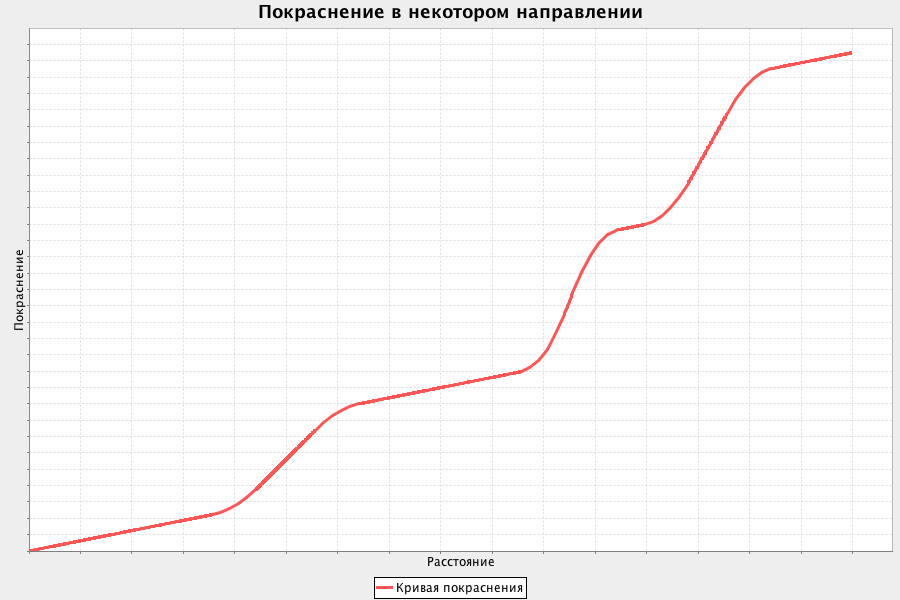
\includegraphics[scale=0.3]{../../presentation/ideal-1-no-tick.png}
			\end{center}        		
        		
        		Где по оси $x$ отложено расстояние по лучу зрения, а по $y$ --- покраснение у соответствующих звезд. Покраснение должно всегда монотонно расти, т.к. везде есть пыль.  Очевидно, что там, где покраснение растет быстрее - пыли больше, там где медленнее - меньше. Поэтому, можно было бы сказать, что облака на этом луче зрения находятся там, где покраснение растет <<очень быстро>> (синие области),   
           
            \begin{center}
           		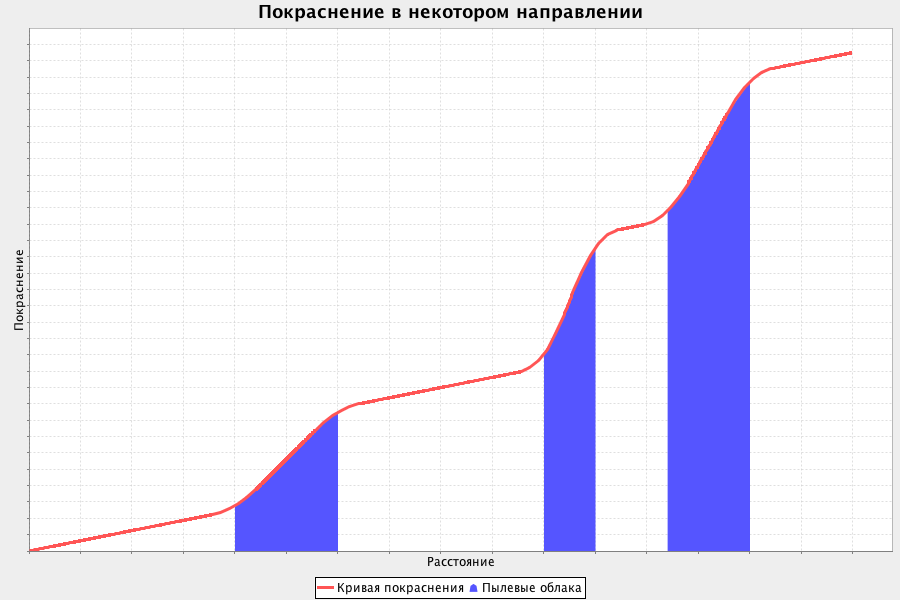
\includegraphics[scale=0.3]{../../presentation/ideal-2-no-tick.png}    
			\end{center}        
        
        		Тем самым, построение кривых покраснения в разных направлениях на небе может позволить находить области повышенного мезвездного поглощения, то есть находить пылевые облака. 
			        
        
        
        %Существуют таблицы <<спектральный класс, класс светимости --- показатель цвета>>, поэтому для каждой звезды из каталога Hipparcos, у которой есть видимый показатель цвета и спектральный класс, можно вычислить покраснение. Если мы для всех таких звезд знаем еще и их пространственные координаты с хорошей точностью, то мы можем говорить о пространственном распределении покраснения. В данной работе мы рассмотрим это распределение с точки зрения трендов покраснения в различных направлениях. Результатом работы будут коэффициенты $a$ и $b$ этих трендов $ar + b$. 
        
        
        
	\section{Способ получения классов светимости}
		%Из каталога (Tycho 2 Sp Types в Hipparcos 2007). Здесь можно рассказать о достоинствах метода автоматического обучения. Обучащающее множество. Качество классификации. III и V классы светимости. Картинки. Результаты дополнения каталога классами светимости.	
	
	    Практически у всех звезд северного полушария, представленных в каталоге Hipparcos, отсутствует класс светимости. Для нас его наличие чрезвычайно важно, ввиду того, что мы на основе класса светимости и спектрального класса мы считаем истинное значение $B - V$ для звезд ($(B - V)_{int}$). Тем самым, отсутствие классов светимости у половины звезд делает невозможным проведение наших расчетов для всего северного полушария.
		
		Исправим это. Рассчитаем неизвестные классы светимости. Сделаем это с помощью методов машинного обучения. Натренируем классификатор, который будет выдавать класс светимости для звезды по двум факторам - показателю цвета и абсолютной звездной величине. Этих факторов будет достаточно, т.к. классы светимости теоретически разделимы на диаграмме Гершпрунга-Рассела. Тренировать классификатор мы будем с помощью метода опорных векторов \cite{svm}.
		
		Доля звезд, которые не относятся ни к III, ни к V классам светимости очень мала (3.6\%, 3354 из 93230). Эти звезды никак на классификацию не влияют. Поэтому, в качестве обучающего множества возьмем звезды только III и V классов с низкими ошибками в расстоянии (не более 3.7\%) и в показателе цвета (не более 0.01). Таких звезд $3634$. Диаграмма Гершпрунга-Рассела с нанесенным на нее обучающим множеством:
		\begin{center}
			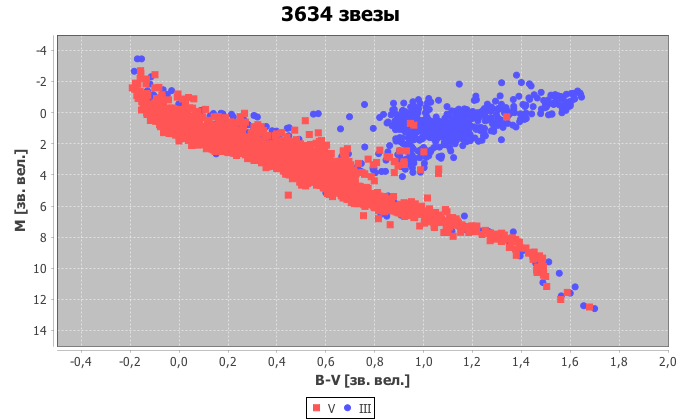
\includegraphics[scale=0.4]{ml-learn.png}   
		\end{center}
        Факторами для обучения у нас будут показатель цвета и абсолютная звездная величина.
		
        Для оценки качества классификатора проведем 10-fold кросс-валидацию. Ниже приведены ее результаты, \\
                
        
        \begin{center}
            \begin{tabular} {| c | c | c | c |}
                \hline
                Классивицированы как $\rightarrow$   &    III   &    V    \\
                \hline
                III    &    656    &    400    \\		
                \hline
                V    &    14    &	2564    \\
                \hline
            \end{tabular}
            \begin{tabular} {| c | c | c | c |}
                \hline
                Класс    &    Точность   &    Полнота    &    F1-мера     \\
                \hline
                III    &    98\%    &    62\%    &    76\% \\		
                V	&	87\%		&	99\%		&	93\%		\\
                \hline
            \end{tabular}
        \end{center}
		 	
        Классификатор, естественно, получился неплохим даже несмотря на то, что многие звезды III класса из обучающего множества ошибочно находятся на главной последовательности (отсюда, низкая полнота у III класса). К подобным каталожным обшибкам мы вернемся в следующей статье.
		 
        Результат работы классификатора --- наличие класса светимости у всех рассматриваемых звезд.
	
    \section{Результаты}
        %Примеры кривой покраснения вписывающихся в теоретическую модель. Обсуждение кривой-прямой. Доверительные интервалы по расстоянию и звездной величине покраснения. Линейная модель покраснения (т.к. просто для других моделей недостаточна точность данных). Распределение коэффициента k по небесной сфере. Сравнение полученного распределения с уже известными данными о пылевых облаках, полученными другими методами (В.Ильин – спросить).	
		
		
        Построение кривых покраснения в разных направлениях позволит нам понять пространственное распределение межзвездного поглощения (пыли). Звезд в каталоге не бесконечное число, поэтому рельные кривые покраснения будут не непрерывными кривыми, а будут наборами точек, описывающими ход покраснения. Аналогично, вместо звезд на луче зрения мы должны использовать звезды в малых конусах. Поэтому, ход покраснения у нас будет выглядеть, к примеру, так,
		\begin{center}
			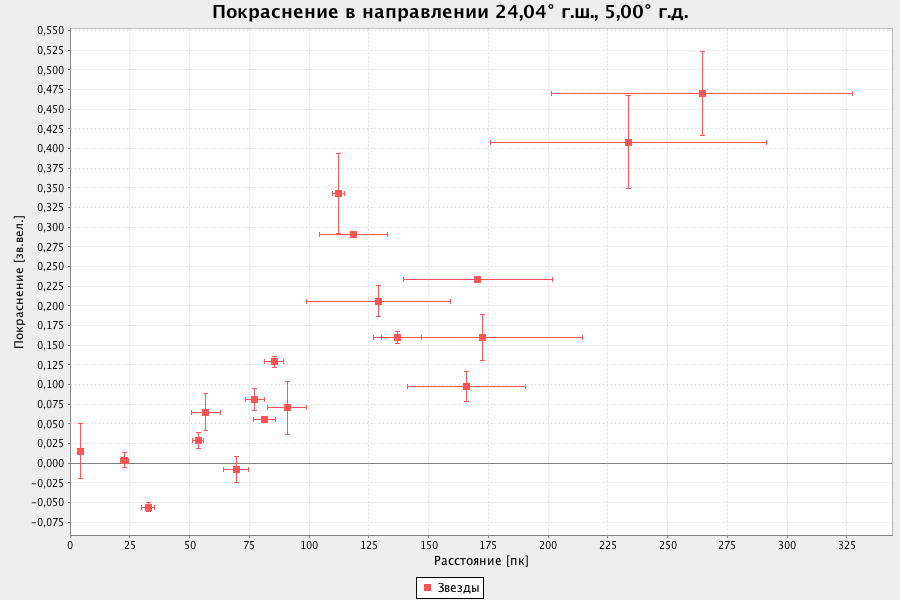
\includegraphics[scale=0.3]{../../presentation/real-1.png}
		\end{center}	
		
        Следующий метод позволит построить <<кривые>> покраснения во всех направлениях на небесной сфере. Он состоит из трех этапов,
        \subsection{Картирование небесной сферы}
            Для картирования небесной сферы мы воспользуемся стандартным алгоритмом Healpix \cite{healpix}, с помощью которого мы разобьем сферу на достаточно маленькие равновеликие части. Назовем их $\{P_i\}_{i = 1}^{2n^2}$ (у нас $n = 18$). Обозначим конусы, высекаемые соответствующими частями через $\{C_i\}_{i = 1}^{2n^2}$\\
			Такое разбиение позволит нам,
            \begin{enumerate}
                \item Рассмотреть ход покраснения в каждом конусе как одномерную функцию $E(r)$. Это корректно, ввиду того, что конусы достаточно узкие;
                \item Сделать наши результаты <<независимыми>>, т.к. конусы не налагаются;
                \item Поместить в каждый конус примерно одинаковое число звезд, чтобы избежать недостатка звезд в некоторых конусах.  
            \end{enumerate}  
		  
	   \subsection{Тренд}
            Тем самым, мы ищем $E_i(r)$, соответствующую каждому $C_i$. Ввиду того, что практически все $E_i(r)$ очень сильно зашумлены разного рода ошибками, не удается проследить истинный ход этих функций. Но тренд вида $k r$ все же можно вычислить ($E_i(r) \approx k_i r$). Он находится с помощью метода наименьших квадратов.  
            
        \subsection{Критерии выбора звезд}
            \subsubsection{По параллаксу}
                В каталоге Hipparcos, далекие звезды имеют очень большие ошибки в параллаксе. На расстояниях, скажем, в 400 пк эти ошибки могут достигать 100\%. Такие ошибки могут очень сильно испортить наши результаты. Тем самым, мы не будем рассматривать звезды, у которых относительная ошибка параллакса не превосходит 25\%. Меньшее значение порога оставит нам очень малое число звезд, которых не хватит для того, чтобы вычисленные тренды были достоверными.
            \subsubsection{По тренду}
                Покраснения некоторых звезд очень сильно портят тренды. Иногда они даже бывают отрицательными, что вообще противоречит здравому смыслу. Но об этом мы поговорим позже.
                
                Как известно, метод наименьших квадратов не устойчив к выбросам, т.е. совсем неверные покраснение/параллакс могут очень сильно испортить тренд. Для более устойчивого построения тренда, мы сделаем следующее. После построения тренда по всем звездам в конусе, мы выбрасываем те, у которых отклонение от тренда самое большое. Затем, мы строим тренд заново, но уже только по оставшимся звездам. После выброса 10\% самых плохих звезд тренд, к примеру, может быть таким
                \begin{center}
					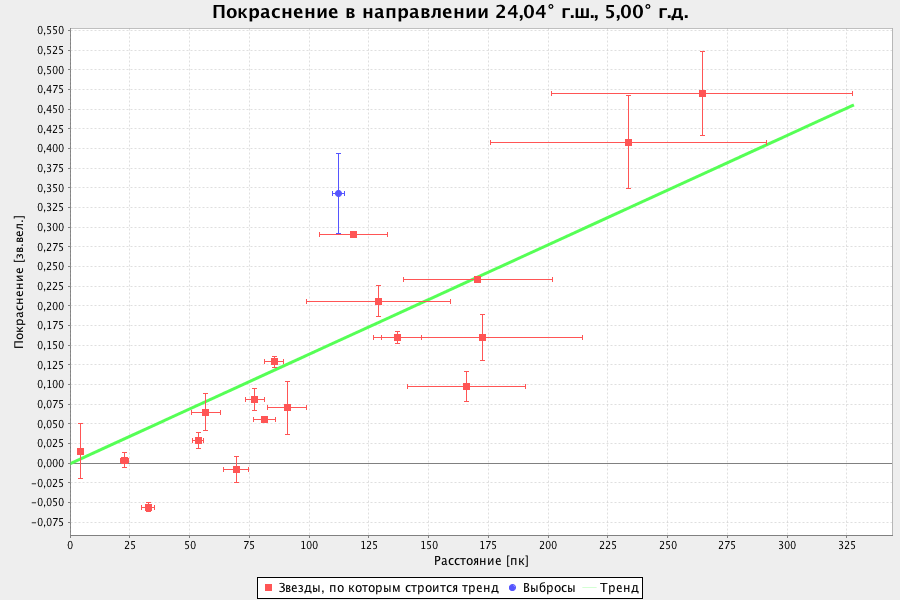
\includegraphics[scale=0.3]{../../presentation/real-2-k.png}
				\end{center}	
                
                В данном случае, мы выбросили одну звезду (синюю). 10\% звезд --- это обычно 0, 1 или 2 звезды в каждом конусе. Опять же, нельзя выкидывать слишком много звезд из-за опасности <<подгонки>> модели. 
		  	 
		  	 
        \subsection{Распределение коэффициента $k$}
            Тем самым, ход покраснения в конусе $C_i$ мы описываем одним числом $k_i$ --- скоростью роста покраснения в этом конусе. Она, как мы ранее выясняли, коррелирует с наличием пыли. Поэтому, составив карту распределения коэффициента $k$, мы составим панораму пыли в окрестности Солнца. 
			\begin{center}
				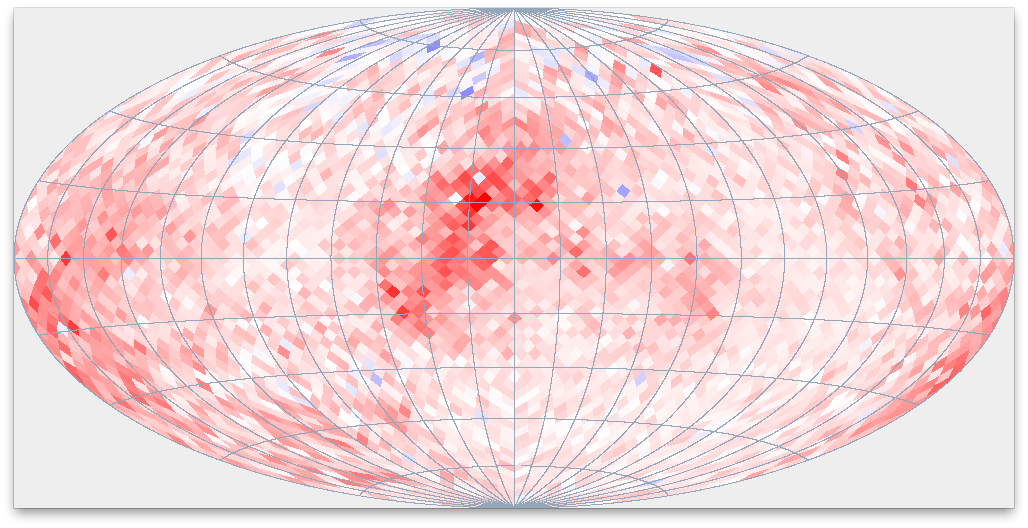
\includegraphics[scale=0.3]{../../presentation/map-k.png}
			\end{center}	
            Это небо в галактической системе координат с центром в центре галактики. Сфера разбита на $12 \cdot 18^2 = 3888$ кусочков алгоритмом Healpix. В каждом кусочке построен тренд покраснения $k r$. На этом рисунке изображено распределение значения коэффициента $k$ по кусочкам. Синий цвет означает отрицательное значение $k$, красный - положительное. Чем насыщеннее цвет, тем больше значение коэффициента по модулю.  
			
	\section{Отрицательное покраснение}
        %Примеры отрицательного поглощения. 1) Существуют звезды с аномальным значением поглощения: значимое отрицательное приращение к показателю цвета. Случайные отклонения, связанные, например, с необычными спектральными характеристиками. 2) Существуют «картинки», в которых целый ряд звезд имеют неправильное поглощение – систематическая ошибка – попытаться выяснить природу. Таблица наиболее значительных отклонений от нормы. Диаграмма.		
	
        На нектороых площадках коэффициент $k$ отрицательный. В теории, такого не должно быть, т.к. межзвездное поглощение не может делать звезды более голубыми. Пример хода покраснения на одной из площадок,
        \begin{center}
            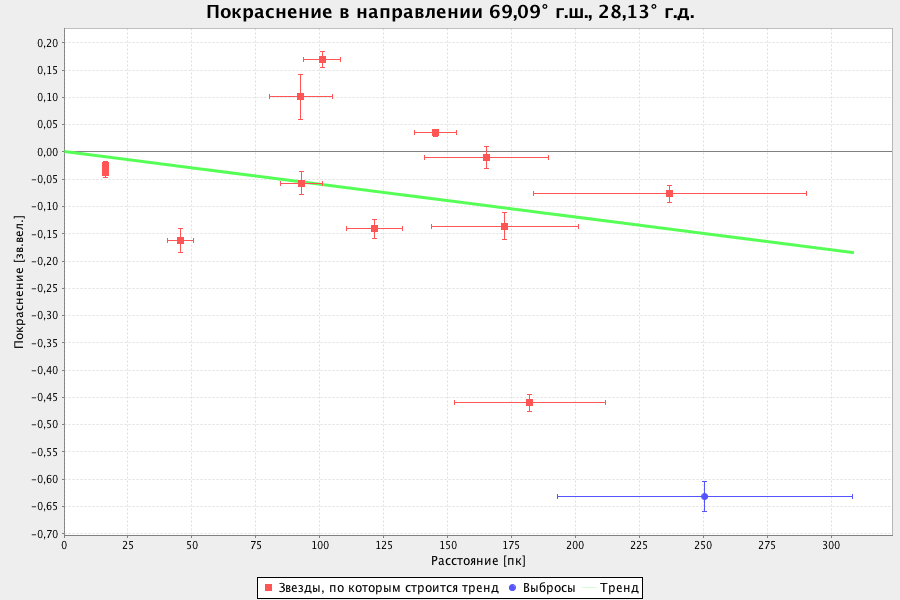
\includegraphics[scale=0.3]{../../presentation/real-4-k.png}
        \end{center}	
        Мы видим, что это вызвано тем, что нектороые звезды имеют сильно отрицательное покраснение. То есть $E_{B - V} + 3 \sigma_{E_{B - V}} < 0$, где $\sigma$ --- это ошибка. Такого не должно быть, т.к. звезда не может сильно голубеть на расстоянии. 
        Давайте рассмотрим какую-нибудь звезду, имеющую такое аномальное отрицательное покраснение. К примеру, HIP 66713. Ее параметры:
        \begin{itemize}
            \item Параллакс $7.99 \pm 0.77$
            \item Показатель цвета $0.386 \pm 0.014$
            \item Спектральный тип G0V
            \item Видимая звездная величина 8.37
        \end{itemize}                
        Мы видим, что у нее нет аномальных параметров. Так же, ее параметры имеют небольшие ошибки. Согласно таблице в \cite{tsvetkov}, спектральному типу G0V соответствует показатель цвета $0.580$. Тем самым, покраснение $E = (B - V)_{obs} - (B - V)_{int} = (0.386 \pm 0.014) - 0.580 = -0,194 \pm 0.014$. Мы видим аномальное покраснение у не аномальной звезды. 
        И таких звезд (имеющих $E_{B - V} + 3 \sigma_{E_{B - V}} < 0$) 11993 из 94670 (12.6\%), то есть достаточно много. Основные возможные причины таких отклонений --- неверные таблицы <<спектральный тип --- покраснение>>, ошибки в спектральной классификации (см. обучающее множество в <<Способах получения классов светимости>>). Этой проблеме будет посвящена следующая статья.  
    
	\section{Заключение} 
        %Получены определенные результаты. Найдены области с большим значением K (красные пиксели). Вопросы: отриц. поглощение – в дальнейшей работе будет проведено исследование.	
	      
	    Этот раздел еще не создан
	      
        
    \begin{thebibliography}{1}
        \bibitem{hipparcos} van Leeuwen, F. {\em Validation of the new Hipparcos reduction}  2007: Astronomy and Astrophysics
        \bibitem{tycho} Wright et al. {\em Tycho-2 Spectral Type Catalog} 2003: The Astronomical Journal
        \bibitem{strigest} Страйджест – книжка
        \bibitem{tsvetkov} А.А.Сминов, А.С.Цветков, А.В.Попов {\em Неточности в спектальной классификации звезд каталога Tycho-2 Spectral Type} 2006.
        \bibitem{goncharov} Гончаров 
        \bibitem{svm} V.N.Vapnik {\em The Nature of Statistical Learning Theory} 1995.
        \bibitem{healpix} Górski et al. {\em HEALPix: A Framework for High-Resolution Discretization and Fast Analysis of Data Distributed on the Sphere} 2005.
    \end{thebibliography}    
\end{document}